% ============================================================
%  ENG4006 BSc Project — Individual Report
%  Youssef Ashraf Othman Abdelrahman (24805073)
%  Project: Echora — AI-Powered Assistive System for Visually
%           Impaired Users
%  Area of responsibility: Perception and AI Models
%
%  BUILD:  tectonic individual_report.tex
%     or:  pdflatex individual_report.tex   (run twice)
%
%  Page 1 is the official UON cover sheet, included from
%  cover_page.pdf (exported from "Cover page.docx").
% ============================================================
\documentclass[12pt,a4paper]{report}

\usepackage[a4paper,margin=1in]{geometry}

% ---- Fonts: Times New Roman look ----
\usepackage[T1]{fontenc}
\usepackage[utf8]{inputenc}
\usepackage{newtxtext}
\usepackage{newtxmath}

% ---- 1.5 line spacing, indented paragraphs ----
\usepackage{setspace}
\onehalfspacing
\setlength{\parindent}{0.5cm}
\setlength{\parskip}{4pt plus 1pt}

% ---- Figures ----
\usepackage{graphicx}
\graphicspath{{images/}}
\usepackage{float}
\usepackage{caption}
\usepackage{subcaption}
\captionsetup{font=small,labelfont=bf,justification=centering}

% ---- Headings ----
\usepackage{titlesec}
\titleformat{\section}
  {\normalfont\bfseries\fontsize{12}{15}\selectfont}{\thesection}{0.6em}{}
\titlespacing*{\section}{0pt}{14pt}{6pt}

% ---- Page numbers bottom-centre ----
\usepackage{fancyhdr}
\pagestyle{fancy}
\fancyhf{}
\fancyfoot[C]{\thepage}
\renewcommand{\headrulewidth}{0pt}
\renewcommand{\footrulewidth}{0pt}
\fancypagestyle{plain}{\fancyhf{}\fancyfoot[C]{\thepage}\renewcommand{\headrulewidth}{0pt}}

\usepackage[hidelinks]{hyperref}
\usepackage{pdfpages}

% Allow long \texttt{} filenames to break rather than overflow the margin.
\sloppy
\setlength{\emergencystretch}{3em}

\begin{document}

% ============================================================
%  PAGE 1 — OFFICIAL UON ASSIGNMENT COVER SHEET
% ============================================================
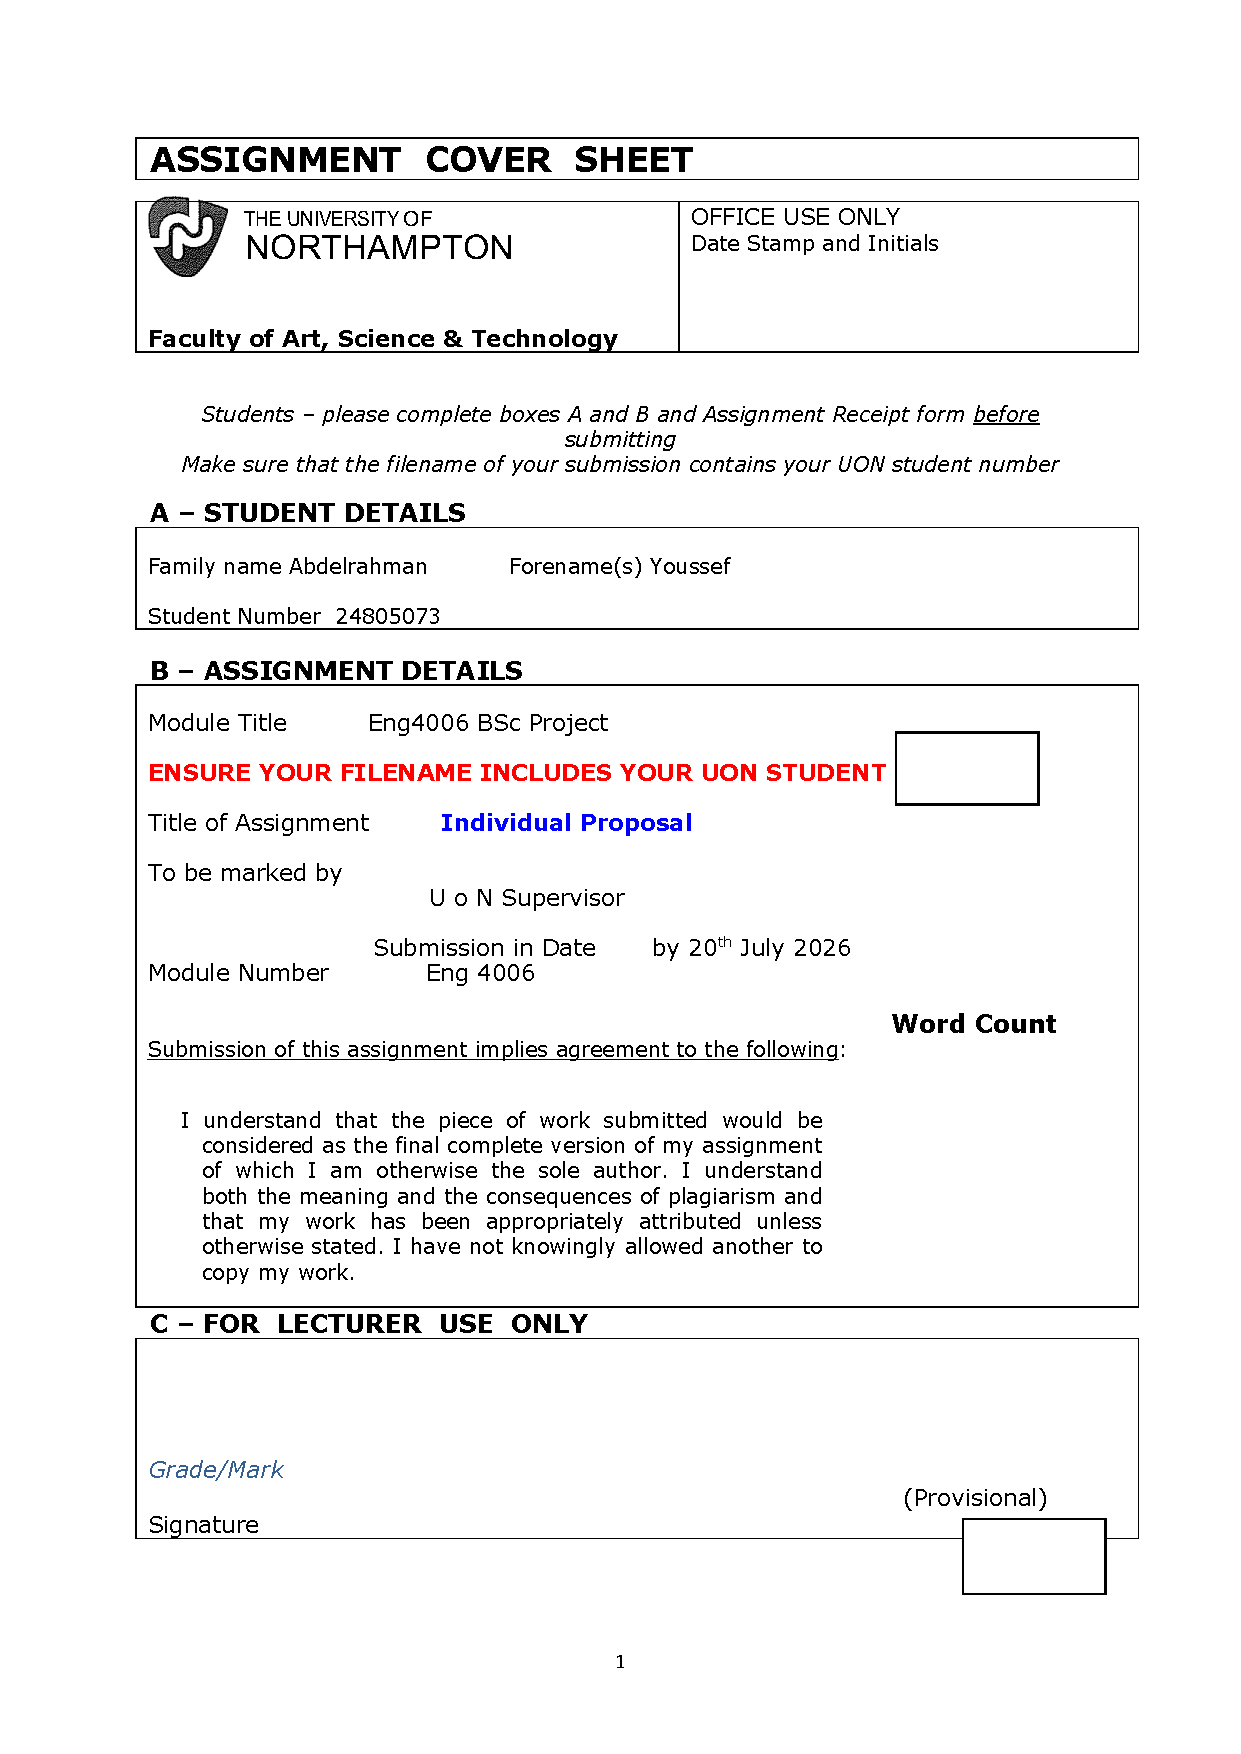
\includepdf[pages=-]{cover_page.pdf}

% ============================================================
%  REPORT
% ============================================================
\pagenumbering{arabic}
\setcounter{page}{1}

\begin{center}
  {\large\bfseries Individual Report}\\[6pt]
  {\normalsize Echora --- An AI-Powered Assistive System for Visually Impaired Users}\\[4pt]
  {\normalsize Area of Responsibility: Perception and AI Models}\\[4pt]
  {\normalsize Youssef Ashraf Othman Abdelrahman --- 24805073}
\end{center}
\vspace{8pt}

% ------------------------------------------------------------
\section*{1. Summary}

Echora is a wearable system that helps blind and low-vision people understand
what is around them. A white cane can tell a person that something is in front of
their feet, but not what that object is, whether it is coming closer, what a sign
says, who has just entered the room, or which banknote is in their hand. Our aim
was to fill that gap with a device that runs completely on the user's own
computer, uses a stereo depth camera, and answers through speech and vibration
instead of a screen.

Our objectives were to build five working modes (navigation, reading, face
recognition, assisted interaction, and money identification), to train our own
models where public ones were not good enough, to stay fast enough for real use,
and to keep all data on the device for privacy. The prototype meets these aims
and runs at about 20 frames per second on ordinary hardware.

My responsibility was the whole perception and AI subsystem. Everything Echora
knows about the world passes through the code I wrote in
\texttt{src/perception/}, so my work sits on the safety-critical path.

% ------------------------------------------------------------
\section*{2. Individual Contribution}

I owned the perception layer end to end: choosing models, preparing datasets,
training, evaluation, tuning for speed, and integration. Figure~\ref{fig:pipeline}
shows the pipeline I built.

\begin{figure}[H]
\centering
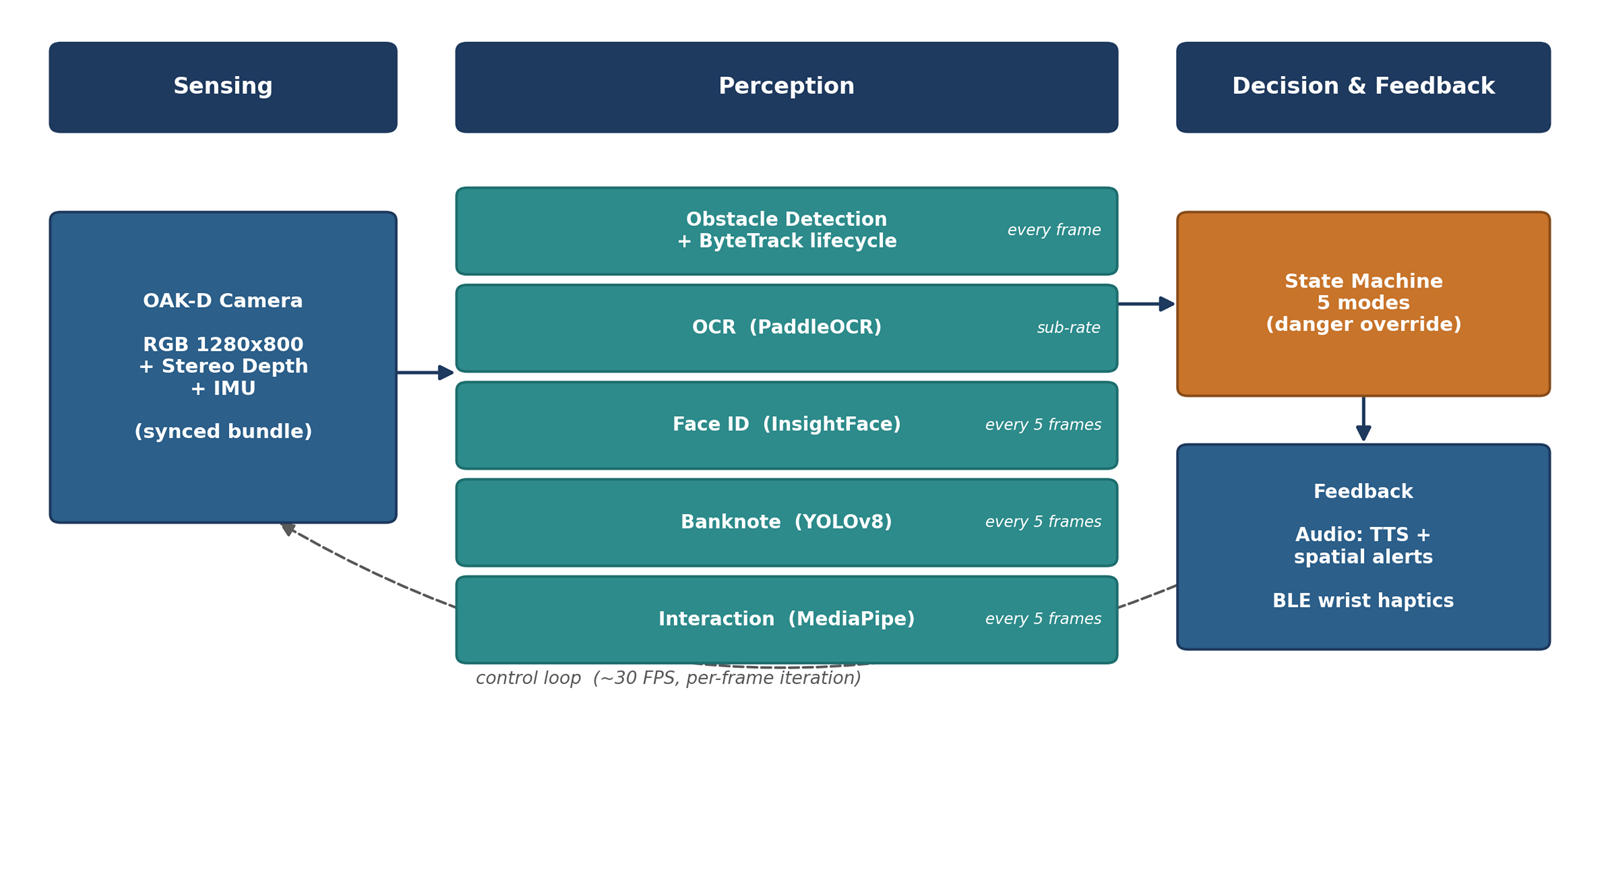
\includegraphics[width=0.88\textwidth]{pipeline.png}
\caption{The perception pipeline I designed: one camera stream feeding five
detection paths, each with its own rate limit and stability check.}
\label{fig:pipeline}
\end{figure}

\noindent\textbf{Obstacle detection.} Navigation is the default mode and the one
where a mistake matters most, so I began there. I chose YOLOv8 because it is
fast enough to warn a walking user in time; two-stage detectors are more accurate
but far too slow. I run \emph{two} YOLOv8s models together: a general COCO model
for everyday things such as people and chairs, and my own accessibility model for
doors, handles, and lift buttons. Since both produce their own track numbers, I
gave each a separate ID range so their tracks can never be confused, and I detect
at $416\times256$ rather than full resolution to protect the frame rate.

For distance, I take the median of the non-zero depth pixels in the middle half
of each box. The median stops one bad pixel from ruining the reading, and using
only the middle avoids picking up the wall behind the object. Each object is then
placed in a zone: danger under 1.5~metres, warning between 1.5 and 3~metres, and
safe beyond that (Figure~\ref{fig:nav}). I added one extra rule: an object inside
the 20-degree corridor straight ahead and closer than 1.8~metres is promoted to
danger, because something in your path is more urgent than something to the side.

\begin{figure}[H]
\centering
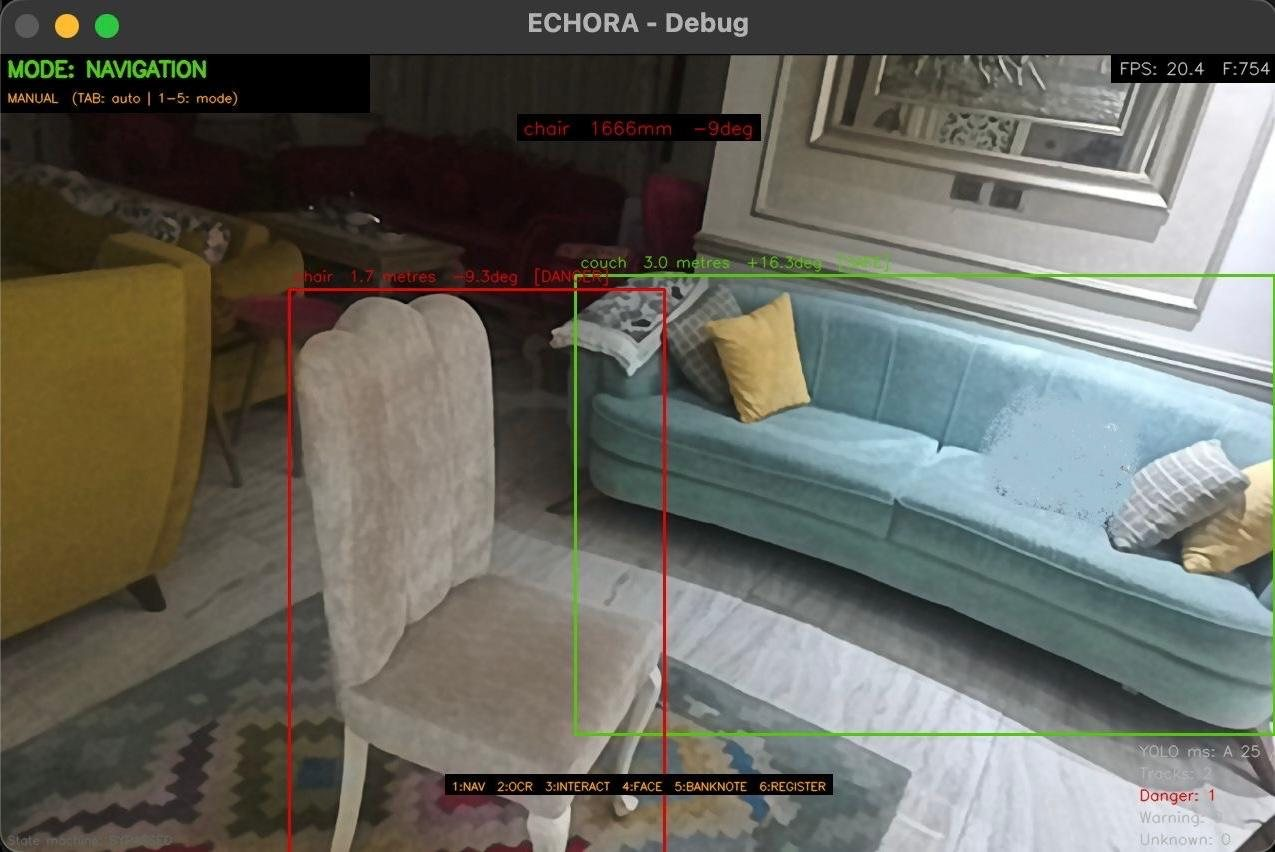
\includegraphics[width=0.78\textwidth]{debug_nav_danger.jpg}
\caption{Live navigation output. Each object shows its class, distance, and
direction, and is coloured by zone.}
\label{fig:nav}
\end{figure}

\noindent\textbf{Tracking.} A detector on its own treats the same chair as a new
object in every frame. I therefore added ByteTrack, choosing it over
appearance-based trackers such as DeepSORT because it follows objects using boxes
alone, with no second network, which protects the frame rate. On top of it I
wrote a small lifecycle layer that I consider one of my better decisions. An
object is trusted only after it has been seen twice, and deleted only after ten
missed frames, so a chair briefly hidden behind a person keeps its identity. I
also estimate speed over a five-frame window to judge whether an object is
approaching. This turns noisy guesses into steady decisions.

\noindent\textbf{Reading text.} For reading I used PaddleOCR's PP-OCRv4. The
default model struggled with real scenes, so I fine-tuned the English recogniser
on the TextOCR dataset. I wrote \texttt{prepare\_textocr\_recognition.py} to cut
out word images and keep only sensible English words. It samples about 12\% of
the data and splits off 5\% for validation, both chosen from a hash of the image
ID rather than at random, so the dataset is exactly reproducible.

I then built two safeguards around the model. The first is adaptive
preprocessing: instead of one fixed filter, the code measures frame brightness
and picks the treatment, giving dark frames strong contrast correction and very
bright frames gamma correction, before sharpening and denoising. The second is a
stability buffer, which speaks text only after it has appeared in three frames.
Without it the system read out momentary mistakes, which is worse than silence
because the user cannot tell the reading was wrong.

\noindent\textbf{Face recognition.} I used InsightFace, pairing RetinaFace for
detection with ArcFace for 512-number embeddings. RetinaFace copes with the odd
angles produced by a camera worn on a moving head, and ArcFace separates people
well from only a few enrolment photos. My main contribution was the matching
rule. Simply accepting the closest match gives confident wrong answers, and
telling a user that a stranger is their friend is a serious failure. So a name
is accepted only if the similarity is at least 0.50 \emph{and} it beats the
second-best person by at least 0.08; if two people are close, Echora stays quiet.
The same name must then appear in a majority of three frames before it is spoken.
To save time, navigation runs only a small $320\times240$ probe, switching to the
full detector when a face is really there.

\noindent\textbf{Datasets, money, and evaluation.} No public dataset of Egyptian
currency existed, so one was built: eleven classes of notes and coins
photographed under different lighting, backgrounds, and angles, with over 7,400
labelled images. Because a wrong answer here costs real money, I set the
confidence threshold high at 0.85, require the same value in three frames, and
only answer when the note is within half a metre. For the accessibility detector
I wrote \texttt{prepare\_accessibility\_yolo\_dataset.py} to merge a door dataset
and a lift-button dataset into one seven-class set, validating every label line.

I then wrote a single script that tests each model on its held-out test split and
reports precision, recall, mAP@0.5, and the stricter mAP@0.5:0.95. The banknote
detector reached mAP@0.5 of 0.991 and mAP@0.5:0.95 of 0.979, with a confusion
matrix that is almost purely diagonal (Figure~\ref{fig:results}). The
accessibility model reached mAP@0.5 of 0.726 with precision of 0.858: doors score
0.913, handles a weaker 0.793 because small objects are harder to locate, and one
class, \texttt{updown}, scores zero recall. That is a data problem, not a model
problem, since there are far too few examples of it. I report it openly because
it points at the fix, which is more data.

\begin{figure}[H]
\centering
\begin{subfigure}{0.48\textwidth}
  \centering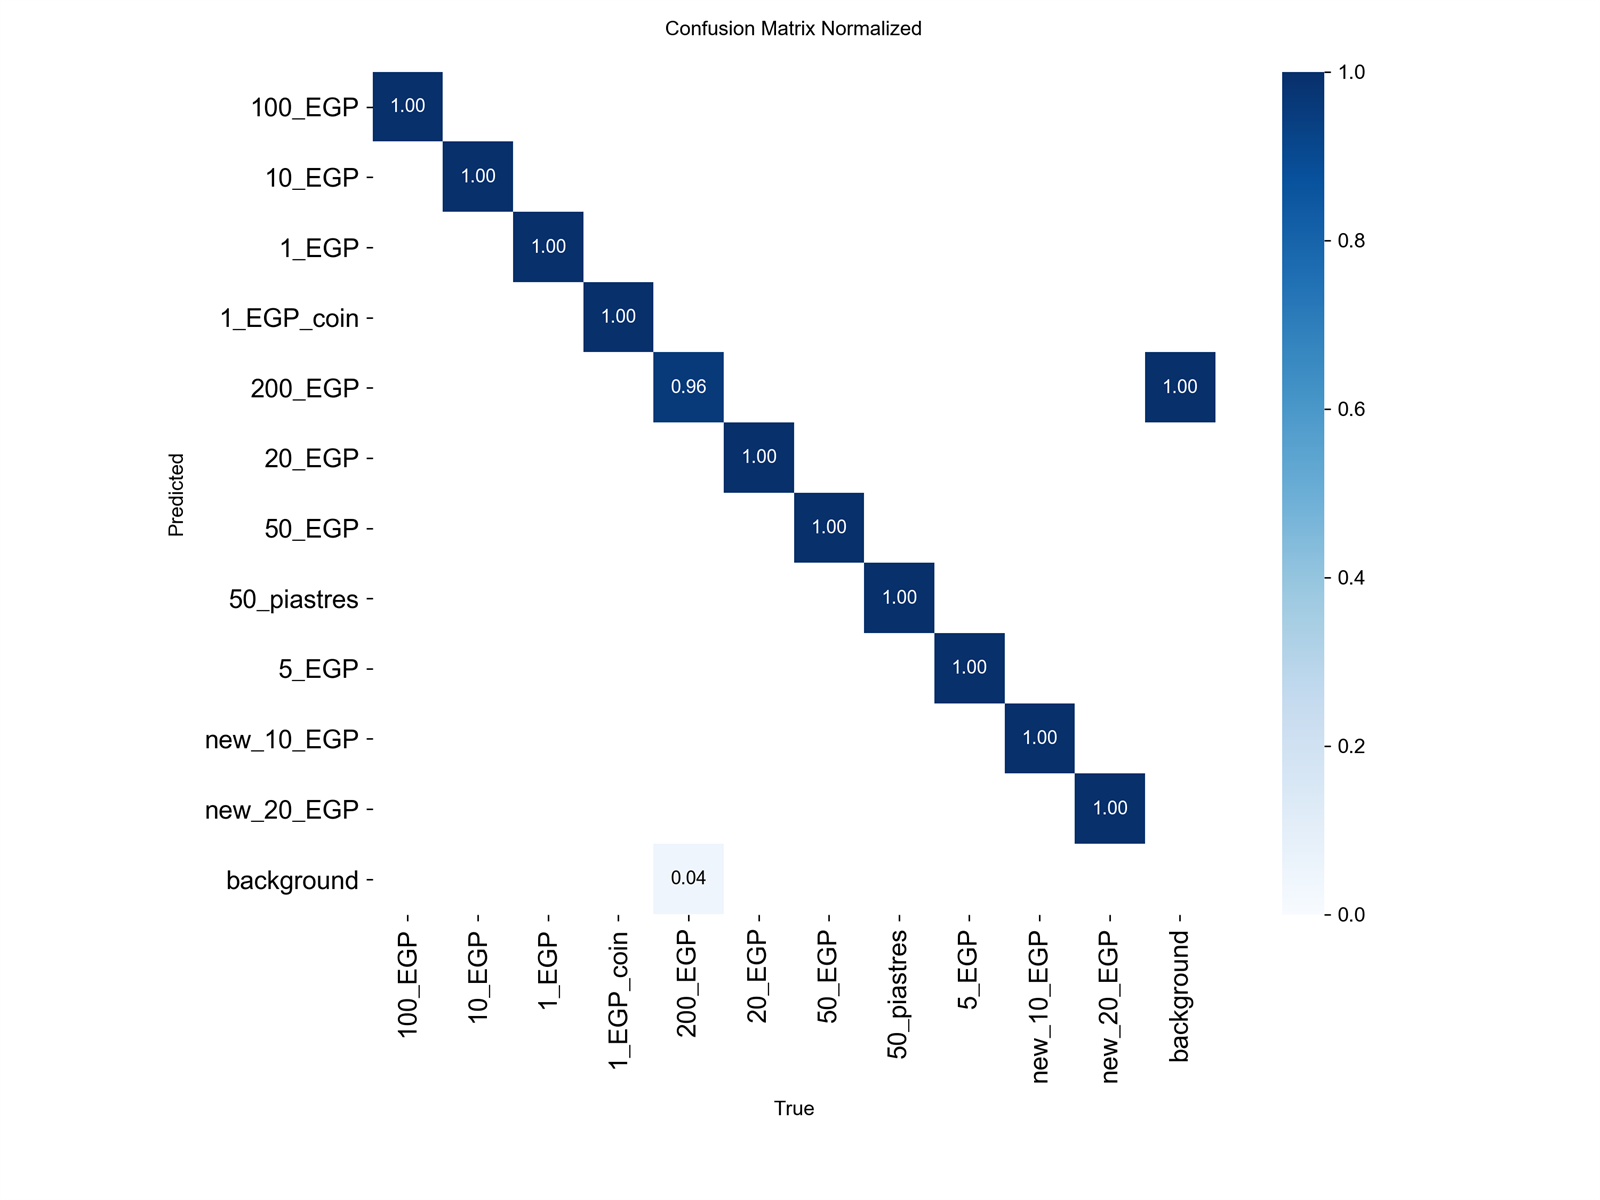
\includegraphics[width=\linewidth]{cm_banknote.png}
  \caption{Banknote detector}
\end{subfigure}\hfill
\begin{subfigure}{0.48\textwidth}
  \centering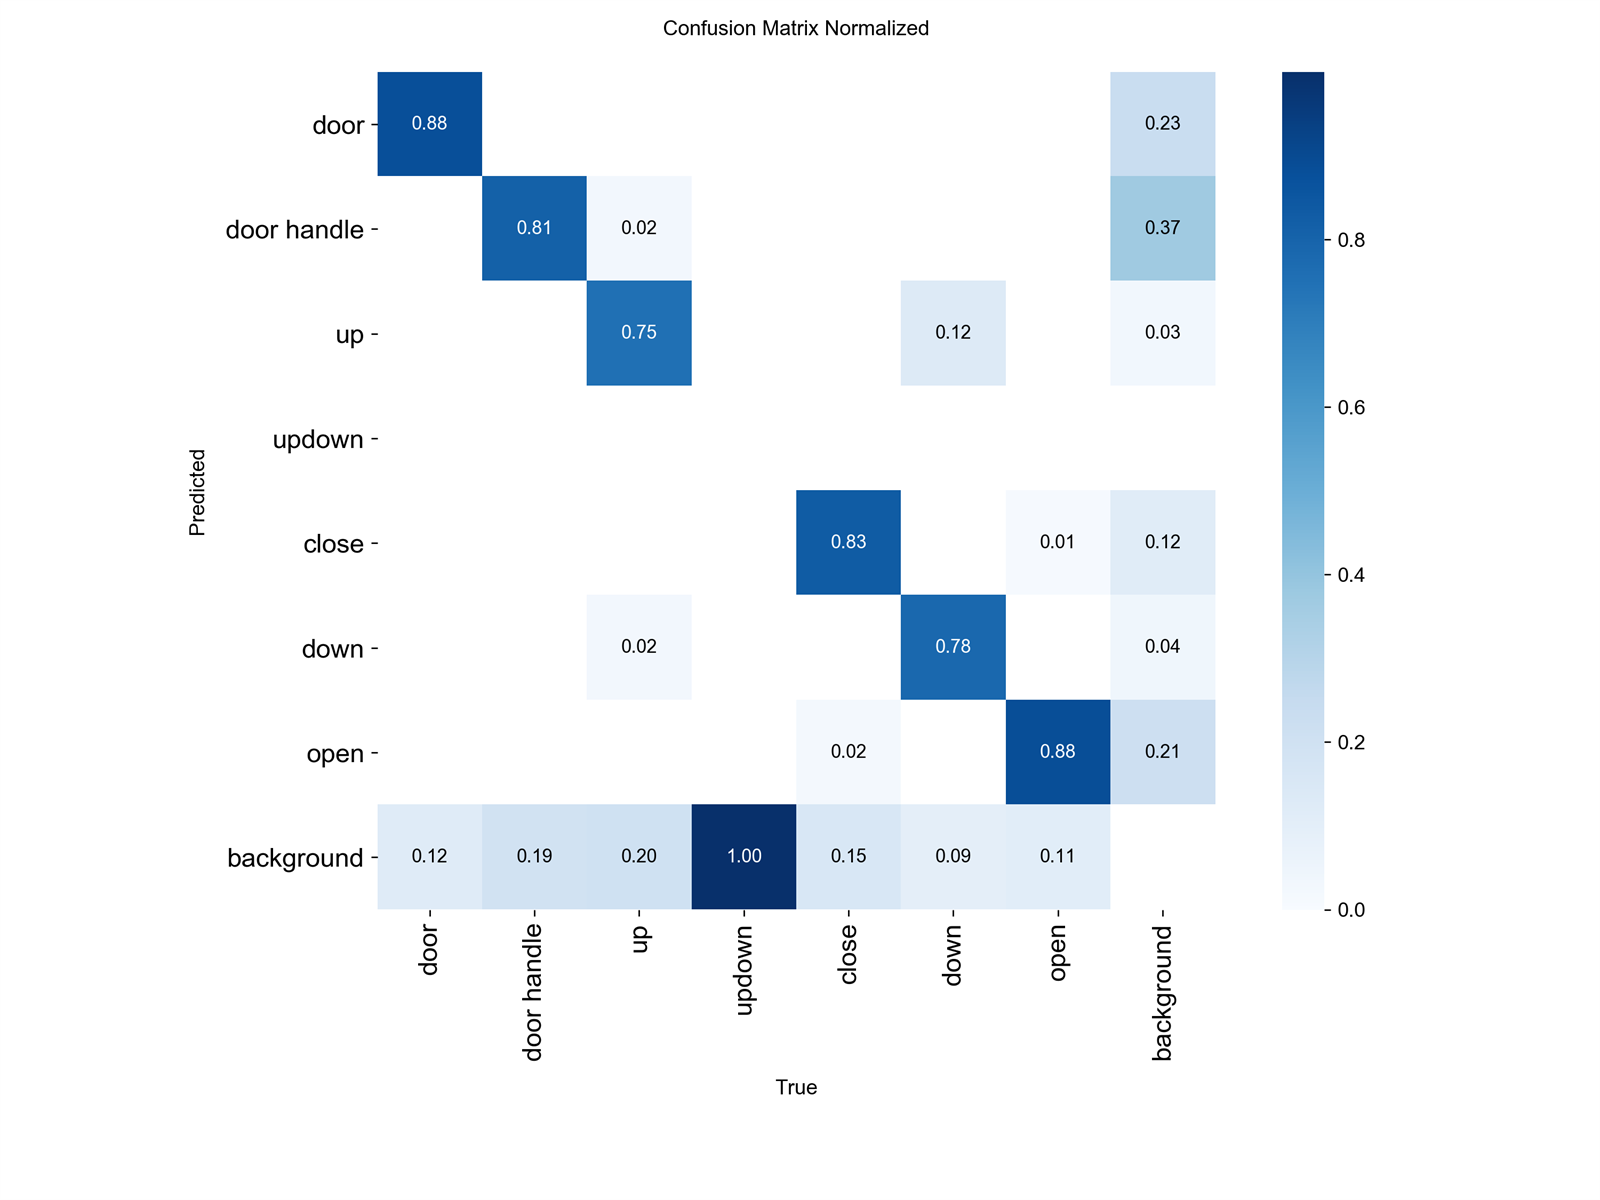
\includegraphics[width=\linewidth]{cm_accessibility.png}
  \caption{Accessibility detector}
\end{subfigure}
\caption{Confusion matrices. The banknote model is almost perfectly diagonal;
the accessibility model shows the weakness in the under-represented classes.}
\label{fig:results}
\end{figure}

\noindent\textbf{Integration and speed.} Running five models at once is very
different from running each alone. I gave every subsystem its own rate: obstacles
run on every frame because safety cannot wait, money every fifth frame, text
every tenth, and faces every fifteenth. I added short-lived caches so two parts
of the code asking the same question in one frame cause only one inference, and
made every module fail safely, so a missing model file or a dropped frame
produces a clear warning instead of a crash.

% ------------------------------------------------------------
\section*{3. Reflection on Project and Progress}

The banknote work went best. Because we collected the data ourselves, we could
deliberately vary lighting and angle, and the near-perfect result taught me
something I now believe strongly: careful dataset design matters more than model
choice. The accessibility detector proved the same point from the opposite side.
Its worst number comes from missing data, and no hyperparameter tuning would have
fixed a class with too few examples. I should have checked class balance first.

Integration was harder than training. Each model worked well alone but they
competed for the GPU together, and my first combined version was too slow. The
fix was structural, not numerical: rate-limit each subsystem, cache repeated
questions, and run a cheap check before an expensive one. This restored real-time
speed without changing a single model.

Using Tuckman's model, our team went through the expected stages. Forming was
slow because we underestimated how tightly perception and feedback were linked.
Storming showed up as an argument about how much the system should say, which I
first settled in favour of saying everything and later, correctly, in favour of
restraint. Once we agreed clear interfaces we normed quickly and performed well
during final integration.

The plan did change. Fine-tuning the OCR model was added when the default proved
too weak, and I trained an indoor detector I finally did not ship because the
merged accessibility model did the job better. Both decisions came from
measurements rather than preference. If I did this again I would write the
evaluation script first, and keep documentation closer to the code; reviewing my
own modules, I found comments describing thresholds I had since changed, exactly
the drift that misleads the next developer.

% ------------------------------------------------------------
\section*{4. Broader Issues}

The most serious ethical issue is face recognition. A worn camera that
recognises people collects data about bystanders who never agreed to anything. My
answer is built into the design: everything runs locally, nothing is sent to any
server, and a person is stored only when the user deliberately enrols them and
types a name, which we treat as consent. This is a real safeguard but not a
complete answer, because the bystander still has no say. I must also record that
the prototype stores face embeddings without encryption. These are biometric data
deserving the same care as passwords, so encrypting them is my next security job.

Bias is a genuine risk. Face recognition models work unevenly across skin tones
and ages, and I did not test this, which is a limitation rather than proof the
problem is absent. Our banknote dataset is deliberately Egyptian, which serves
our users well but does not transfer elsewhere.

Reliability matters differently in each direction. A false alarm is annoying; a
missed obstacle can mean a collision. My tracking rules, high money threshold,
and cautious face margin all trade a little speed for fewer confident mistakes.
Echora is offered as a companion to the white cane, never a replacement.

Training is the project's largest energy cost. Fine-tuning from pretrained
weights rather than training from scratch cut that a lot, and running on an
ordinary computer rather than in the cloud keeps everyday use low.

Finally, building for vulnerable users raises the professional bar. A blind user
often cannot check what the system tells them, so dependability and honesty are
duties rather than features. Reporting our weak results as openly as our strong
ones is part of that same responsibility.

\end{document}
